\begin{figure}[t]
  \centering
  \usetikzlibrary{shapes.arrows}
  \definecolor{tile0}{HTML}{DABDE4}
  \definecolor{tile1}{HTML}{B8DBF4}
  \definecolor{tile2}{HTML}{B5EDCD}
  \definecolor{tile3}{HTML}{FBEBA7}
  \definecolor{tile4}{HTML}{F9C1BB}


  \tikzstyle{array_element}=[rectangle,
                             minimum height=1.0cm, 
                             minimum width=1.0cm, 
                             minimum size=1.0cm,
                             draw=gray,
                             rounded corners=2.5 ]


  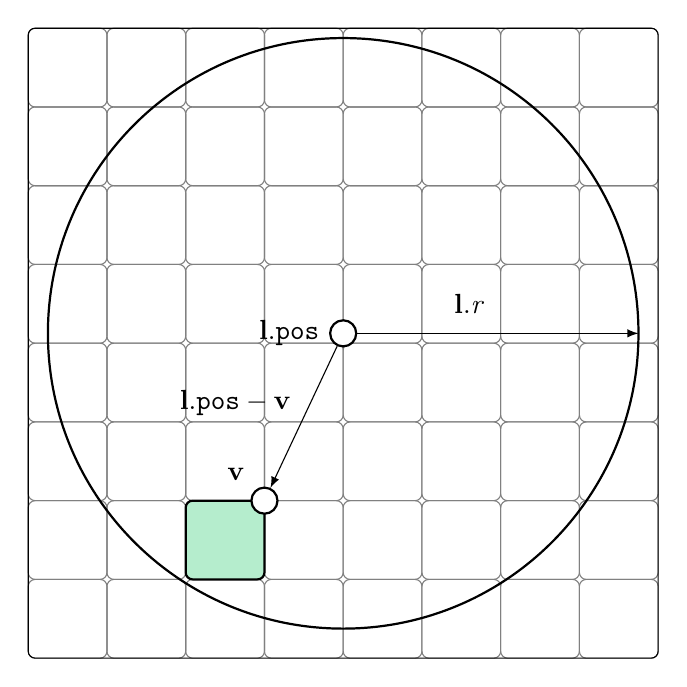
\begin{tikzpicture}
    \foreach \la in {0,...,7} {
        \foreach \lb in {0,...,7} {
            \node at (1.0cm * \la, 1.0cm * \lb) () [array_element] {};
        }
    }
    \node at (1.0cm * 2, 1.0cm ) () [array_element, fill=tile2, draw=black, thick] {};
    \node at (3.5cm, 3.5cm) () [rectangle, minimum size=8cm, draw, rounded corners=2.5,] {};
    \node at (3.5cm, 3.625cm) (UC1) [circle, draw, minimum size=7.5cm, thick] {};
    
    \node at (3.5cm, 3.625cm) (lc) [circle, draw, minimum size=0.1cm, thick, fill=white, label=west:{$\mathbf{l}.\mathtt{pos}$}] {};
    \node at (3.5cm + 3.75cm, 3.625cm) (lr) [] {};
    \draw[-latex] (lc) -- (lr.center) node[pos=0.4, label=north:{$\mathbf{l}.\mathit{r}$}] {};
    
    \node at (0.5cm + 1.0cm * 2, 0.5cm + 1.0cm) (la) [circle, draw, minimum size=0.1cm, thick, fill=white, label=north west:{$\mathbf{v}$}] {};
    \draw[-latex] (lc) -- (la) node[pos=0.4, label=west:{$\lVert \mathbf{l}.\mathtt{pos} - \mathbf{v}  \rVert$}] {};
  \end{tikzpicture}
  \caption{Bepaling of een knoop overlapt met het lichtvolume.}
  \label{fig:hs-light-grid}
\end{figure}

